%!TEX root = ../thesis.tex

\chapter{Grundlagen}
\label{chap:fundamentals}
\todo{Grundlagen einteilen und schreiben}
In diesem Kapitel werden die Grundlagen erläutert, die für das Verständnis dieser Arbeit wichtig sind. 

Zum einen werden in \prettyref{sec:darts} die Grundlagen des Dartsportes erläutert, auf deren Wesen die Idee dieser Abhandlung fußt. Dabei wird vom Dartboard bis zu den Darts und den allgemeinen Turnierregeln ein Überblick gegeben, um den Nutzen und die Motivation verständlicher zu machen.

Anschließend wird im \prettyref{sec:setup} das genutzte Testsetup dargestellt, welche für die praktische Implementierung genutzt wird.

Weiterhin werden grundlegende Informationen der Bildverarbeitung vermittelt im \prettyref{sec:basics}. Es wird ebenfalls ein Überblick über die verwendeten Bibliotheken zur Implementierung gegeben.
\section{Dartsport}
\label{sec:darts}
Der Dartsport hat im Jahr 1920 eine erste Standardisierung erhalten. Die 1924 gegründete National Dart Association hat diesen zum Standard ihrer Liga erklärt \autocite[Chapter 1]{guide2013}. Diese Standardisierung findet sich in vielen heutigen Regelwerken der verschiedenen Verbänden wieder. Auch in der Sport- und Wettkampfordnung des Deutschen
Dart-Verband (DDV) \autocite{DartsRegel2016}.

\begin{figure}
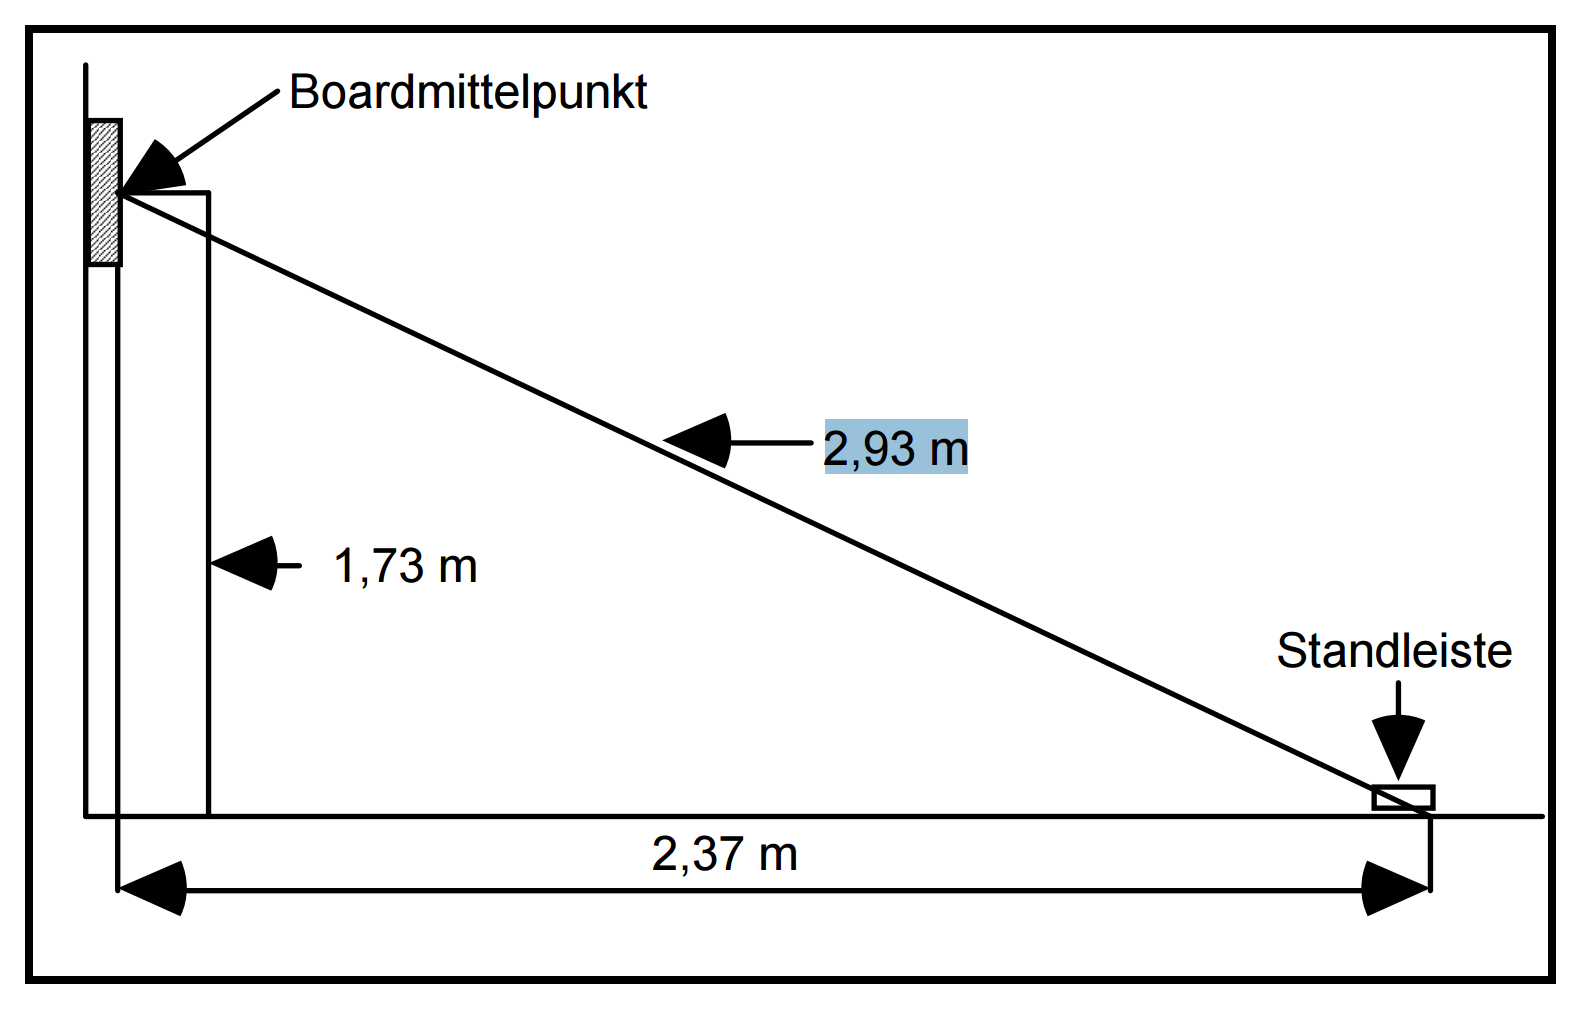
\includegraphics[width=\textwidth]{media/Dartsfield}\\
\caption{\textbf{Seitenansicht von Board und Standleiste 
\cite[8]{DartsRegel2016}}
}
\label{Fig:darts}
\end{figure}

\begin{figure}
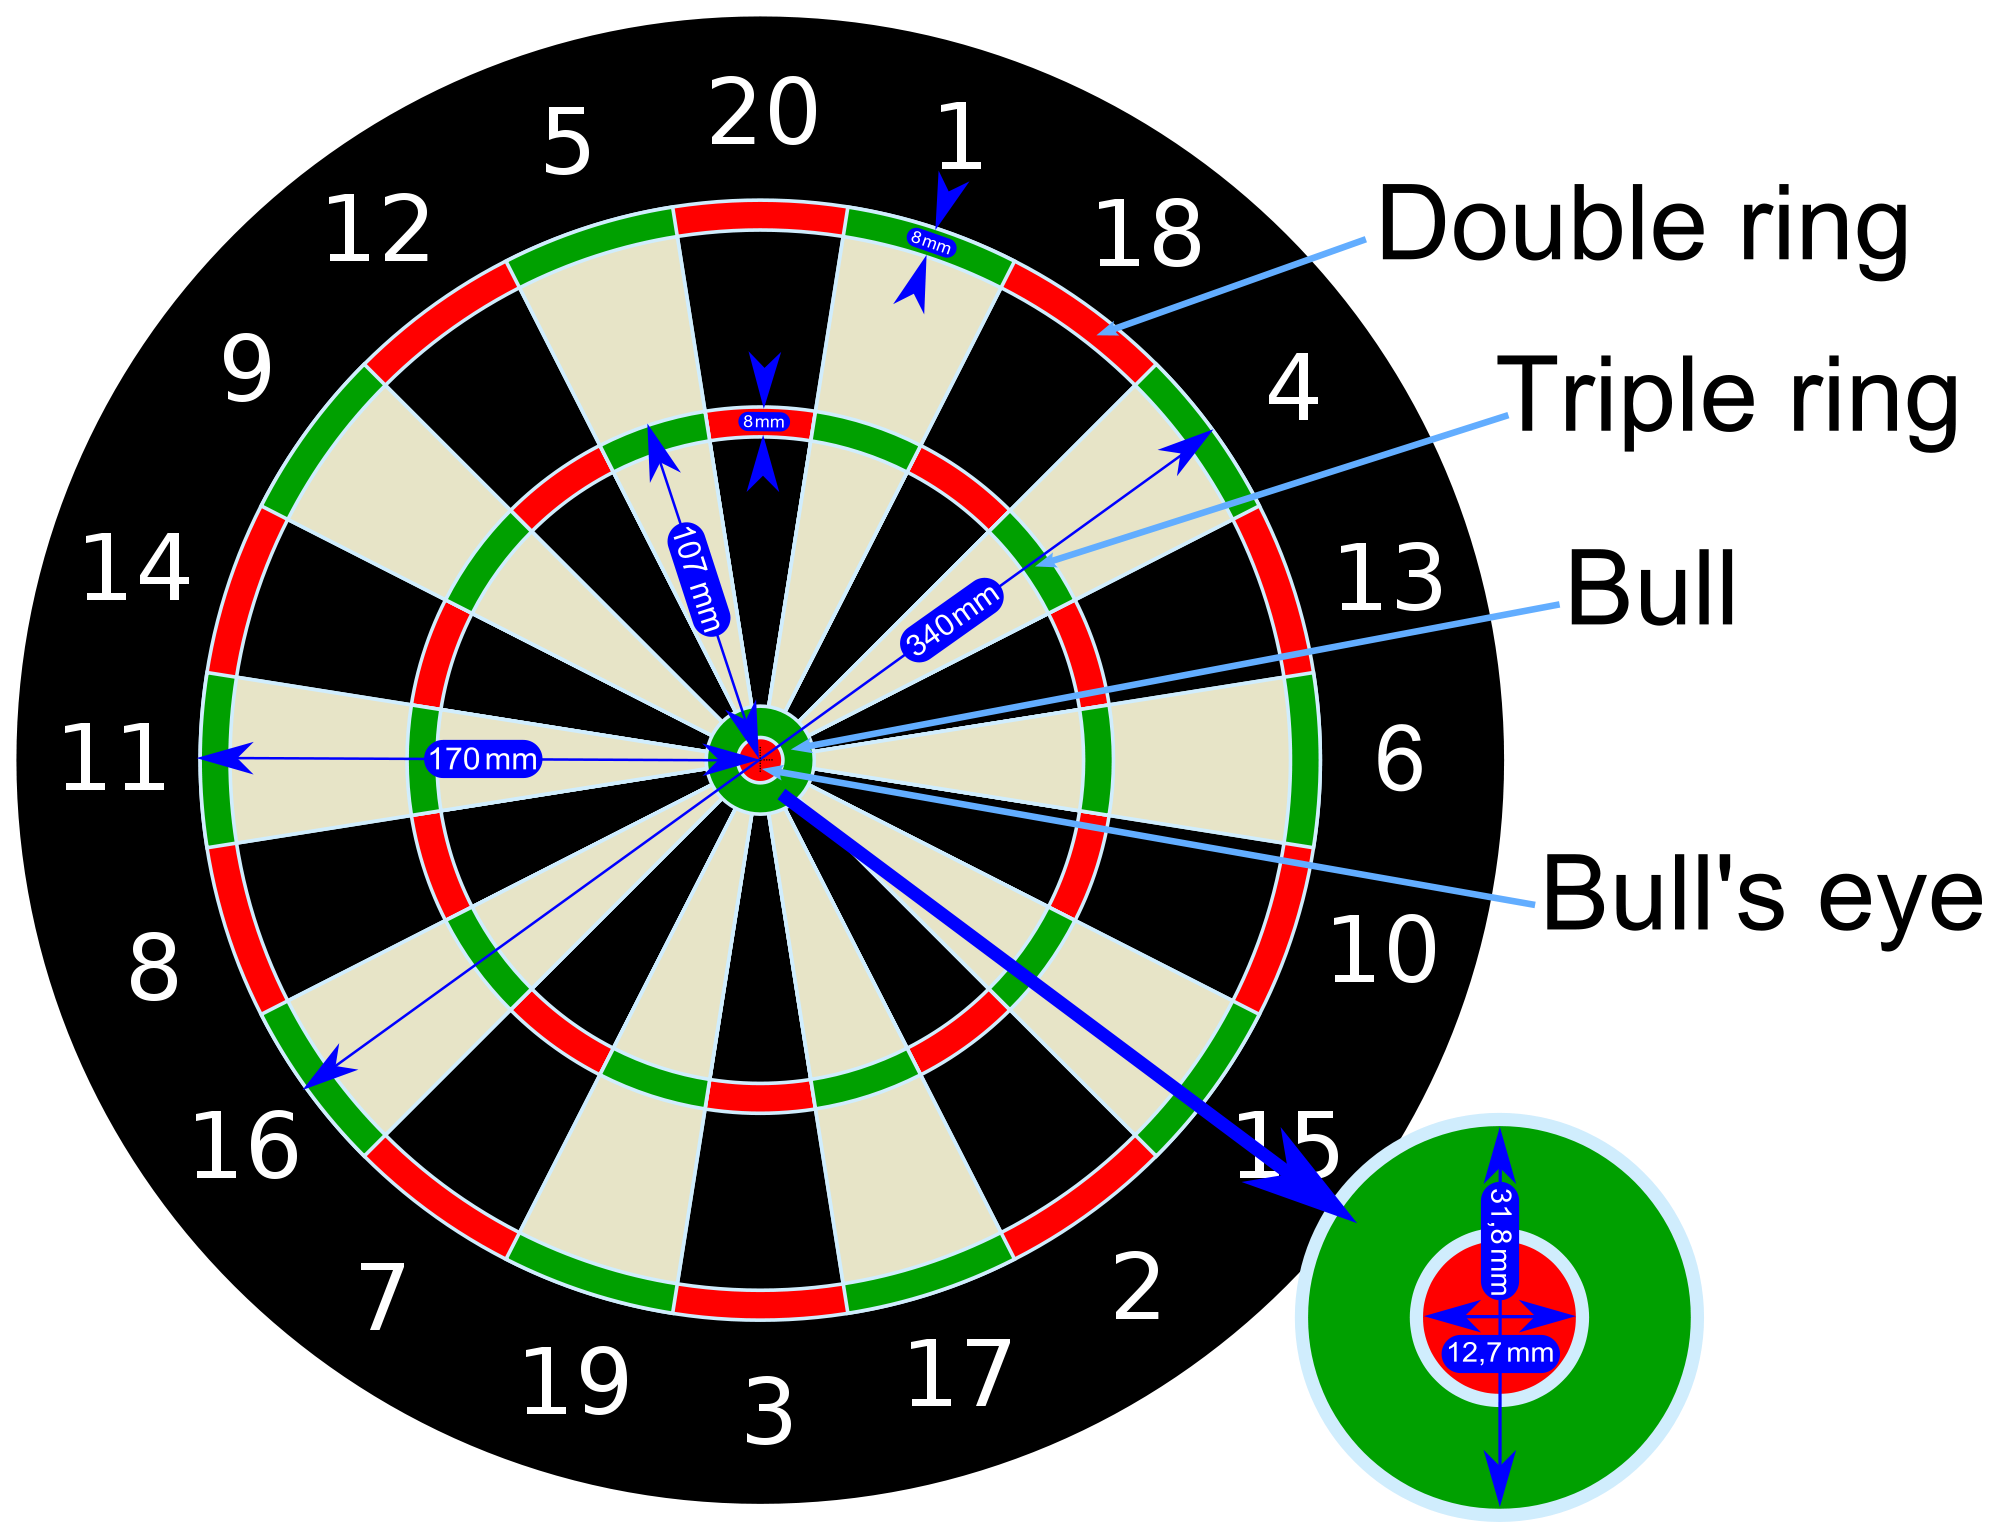
\includegraphics[width=\textwidth]{media/Dartboard_Abmessungen}\\
\caption{\textbf{Standardisiertes Dartboard\cite{Board2016}}
}
\label{Fig:darts}
\end{figure}

\begin{figure}
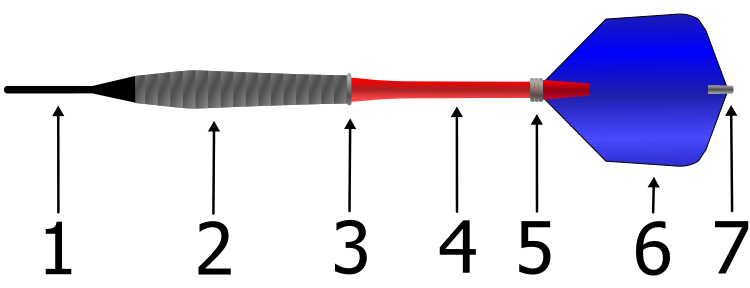
\includegraphics[width=\textwidth]{media/Dart}\\
\caption{\textbf{Aufbau eines Darts\cite{dart2006}}
}
\label{Fig:darts}
\end{figure}

\section{Aufbau der Testumgebung}
\label{sec:setup}

\section{Grundlagen Bildverarbeitung}
\label{sec:basics}
Das Pinhole Camera Modell sieht wie folgt aus: \autocite{Zhang2000}.
\begin{figure}
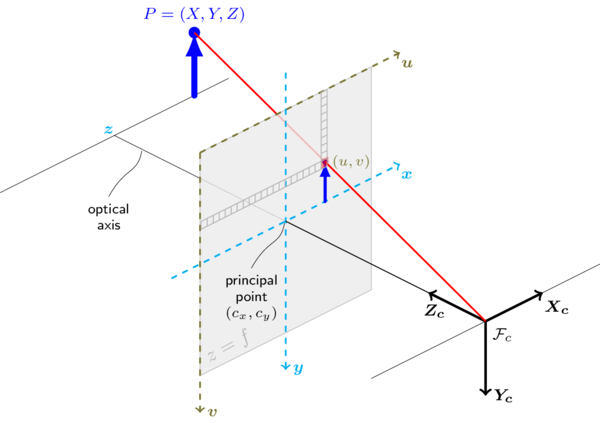
\includegraphics[scale =0.75]{media/pinhole_camera_model}\\
\caption{\textbf{Pinhole Camera Modell von.\autocite{OpencvCamera2016}}
}
\label{Fig:pinhole}
\end{figure}


\todo{pinhole Camera Modell erläutern}
\todo{opencv Benutzung erklären}
OpenCV ist eine \autocite[512--]{Medioni:2004:ETC:993884}

